
\subsubsection{A. Bootstrap Slope Distribution}

\begin{figure}[htbp]
\centering
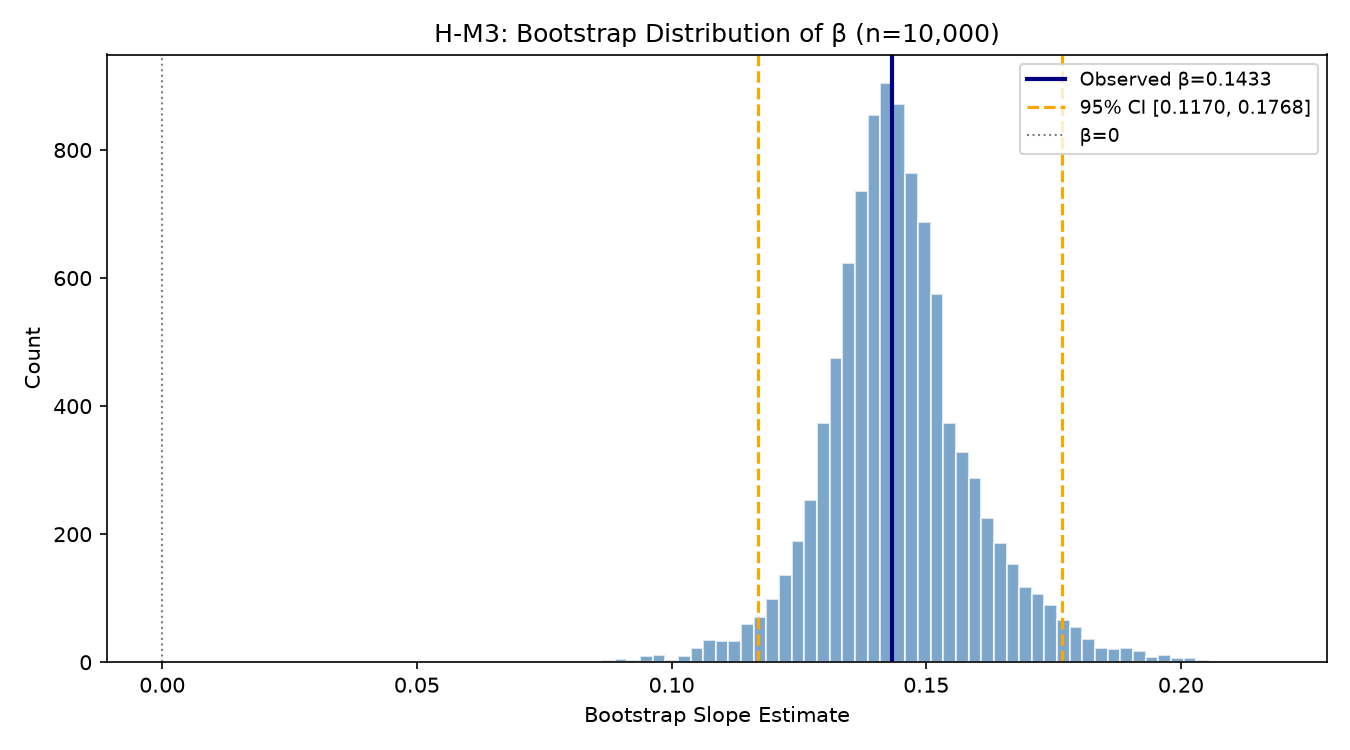
\includegraphics[width=\columnwidth]{figures/bootstrap_histogram.png}
\caption{Bootstrap histogram}
\label{fig:bootstrap_histogram}
\end{figure}

\textit{Figure 8: Bootstrap slope distribution for Coste et al. data (N = 10,000 iterations, seed = 42). Distribution is unimodal and approximately Gaussian, centered at $\beta \approx$ 0.143. Bootstrap CI [0.117, 0.177] is strictly positive.}

\subsubsection{B. Gao et al. Dual-Axis Trajectory}

\begin{figure}[htbp]
\centering
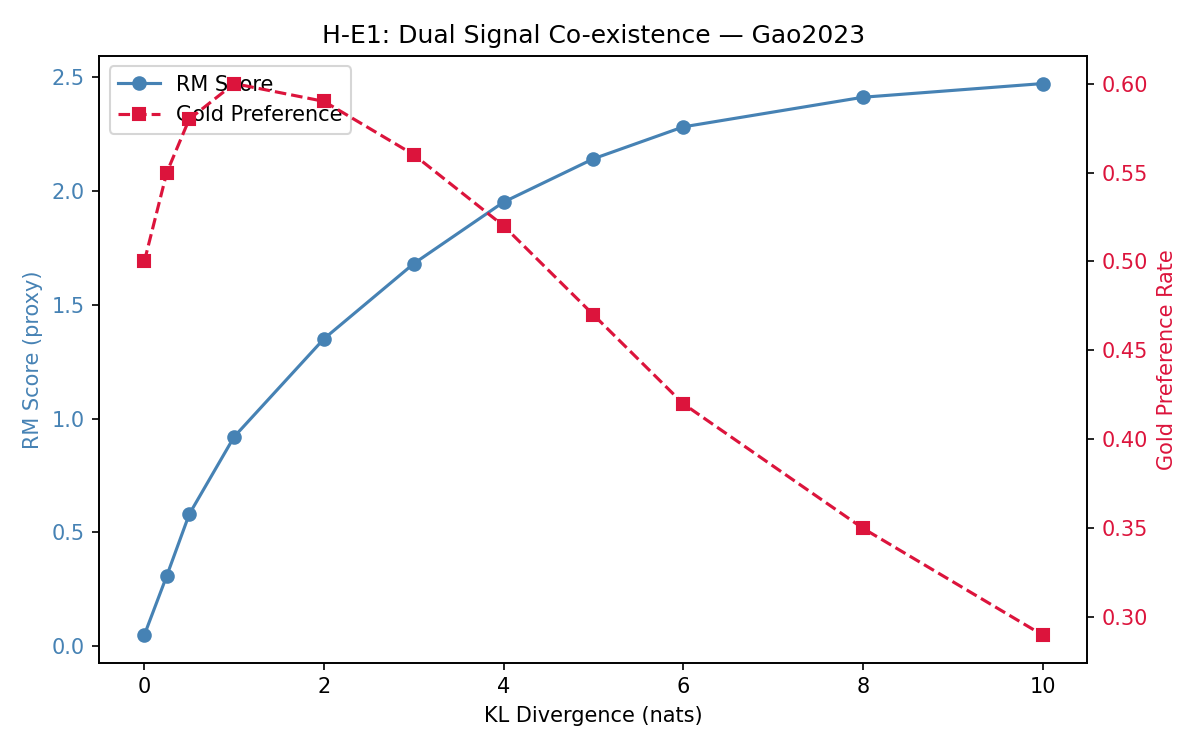
\includegraphics[width=\columnwidth]{figures/dual_axis_gao2023.png}
\caption{Dual-axis Gao 2023}
\label{fig:dual_axis_gao2023}
\end{figure}

\textit{Figure 9: Dual-axis trajectory for Gao et al. [2023] across all 11 available KL levels (including the KL = 0 boundary point used for signal characterization in H-E1). Unlike Coste et al. data, the gap is initially negative at low KL (gold preference rises faster than RM), crosses zero at ~3.5 nats, then enters the positive regime. The regression (H-M4) uses n = 10 observations (KL = 0 boundary point excluded).}

\subsubsection{C. Full Regression Summary --- Coste et al. [2023]}

\begin{verbatim}
OLS Regression Results (statsmodels)
Dep. Variable:  gap           R-squared:      0.958
N:              10            Adj. R-squared:  0.952
F-statistic:    181.2         Prob (F):        8.89e-07

Coefficients:
  const   -0.4016   (t = -8.344, p = 0.000)  [CI: -0.513, -0.291]
  KL       0.1433   (t = 13.461, p = 0.000)  [CI:  0.119,  0.168]

Omnibus: 1.751 (p = 0.417)  Durbin-Watson: 0.411  Jarque-Bera: 0.868 (p = 0.648)
\end{verbatim}

\subsubsection{D. Full Regression Summary --- Gao et al. [2023]}

\begin{verbatim}
OLS Regression Results (statsmodels)
Dep. Variable:  gap           R-squared:      0.701
N:              10            Adj. R-squared:  0.663
F-statistic:    18.74         Prob (F):        0.00251

Coefficients:
  const   -0.4960   (t = -3.795, p = 0.005)  [CI: -0.797, -0.195]
  KL       0.1599   (t =  4.329, p = 0.003)  [CI:  0.075,  0.245]

Omnibus: 1.658 (p = 0.436)  Durbin-Watson: 0.436  Jarque-Bera: 0.913 (p = 0.633)
\end{verbatim}
